\documentclass[10pt]{beamer}
\usetheme[progressbar=frametitle]{metropolis}
\usepackage{appendixnumberbeamer}
\usepackage{booktabs}
\usepackage{makecell}
\usepackage{multicol}
\usepackage{xspace}
\usepackage{emoji}
\usepackage[backend=biber,style=alphabetic]{biblatex}

\addbibresource{references.bib}
\ExecuteBibliographyOptions{isbn=false,url=false,doi=true,eprint=false}
\DeclareSourcemap{
  \maps[datatype=bibtex, overwrite]{
    \map{
      \step[fieldset=editor, null]
      \step[fieldset=booktitle, null]
      \step[fieldset=series, null]
      \step[fieldset=pages, null]
      \step[fieldset=address, null]
      \step[fieldset=journal, null]
      \step[fieldset=publisher, null]
      \step[fieldset=volume, null]
      \step[fieldset=number, null]
      \step[fieldset=note, null]
    }
  }
}

\def\do#1{
  \DeclareBibliographyDriver{#1}{%
    \usebibmacro{bibindex}%
    \usebibmacro{begentry}%
    \usebibmacro{author/editor+others/translator+others}%
    \setunit{\labelnamepunct}\newblock
    \usebibmacro{title}%
    \newunit\newblock
    \usebibmacro{date}%
    \newunit\newblock
    \iftoggle{bbx:doi}
      {\printfield{doi}}
      {}%
    \setunit{\bibpagerefpunct}\newblock
    \usebibmacro{pageref}%
    \newunit\newblock
    \usebibmacro{finentry}}}
\makeatother


\newcommand{\PresQ}[0]{\textsc{PresQ}\xspace}
\newcommand{\eqdist}{\stackrel{d}{=}}

% 2. El acto consistirá en la exposición oral por el doctorando del trabajo de
% investigación elaborado ante los miembros del tribunal, refiriéndose
% principalmente a la labor realizada, la metodología, el contenido y las conclusiones,
% haciendo especial mención de sus aportaciones originales.

% Evaluación
% i. Justificación del carácter innovador del tema de estudio.
% ii. Adecuación de la metodología utilizada o propuesta de alternativas
% iii. Grado de claridad en la exposición de los resultados obtenidos y análisis de los mismos.
% iv. Observación de la correcta elección y citación de la bibliografía.
% v. Análisis crítico de las conclusiones de estudio.

% Creo que las mismas secciones que la tesis, pero tampoco es plan de ser redundante?

\title{Navigating Diverse Datasets\\
in the Face of Uncertainty}
\subtitle{}
\date{September 11, 2023}
\author{Alejandro Álvarez Ayllón}
\institute{
Tesis dirigida por Dr. Juan Manuel Dodero Beardo y Dr. Manuel Palomo Duarte \\
Programa Oficial de Doctorado en Ingeniería Informática de la Universidad de Cádiz
}
\titlegraphic{\hfill
\includegraphics[height=1.5cm]{uca-logo.pdf}}

\begin{document}

\maketitle

\section{Introduction}

\begin{frame}{Motivation}
\begin{enumerate}
    \item Data exploration represents the fourth paradigm of scientific exploration, alongside experimental, theoretical, and computer-simulation paradigms.
    \item Data exploration is a vital component of the data-intensive scientific process.
    \item Researchers must curate, understand, and extract information from data sets.
    \item To extract knowledge, first, they need to identify patterns: \alert{data mining}.
\end{enumerate}
\end{frame}

\begin{frame}{}
\begin{figure}
    \centering
    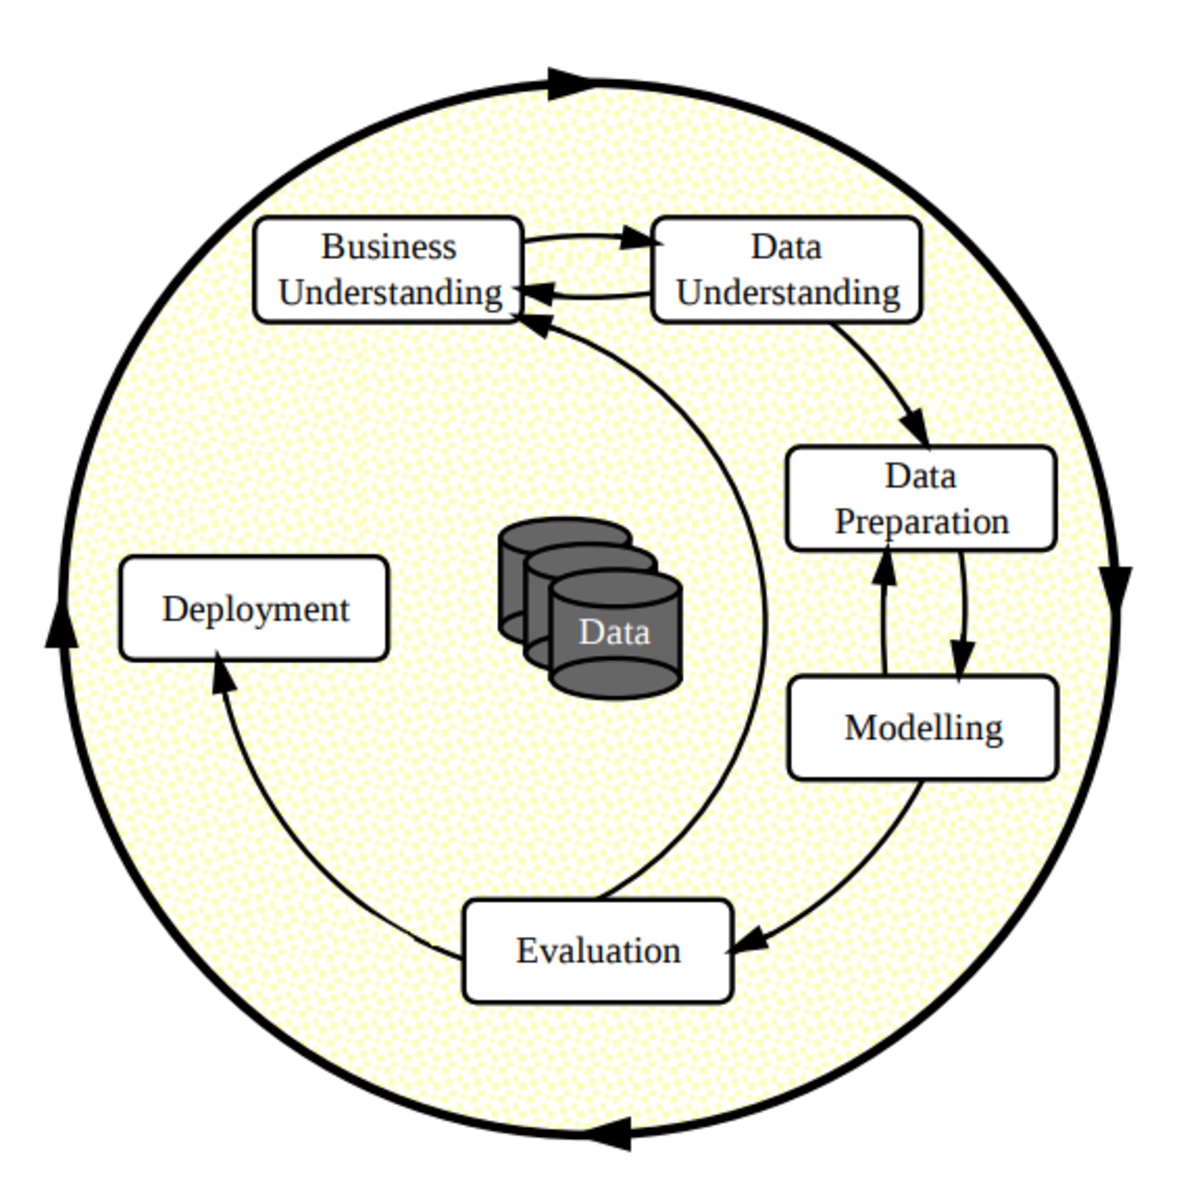
\includegraphics[height=0.8\textheight]{crisp-dm.pdf}
    \caption{CRoss Industry Standard Process for Data Mining}
\end{figure}
\end{frame}

\begin{frame}{Our Focus: Data Understanding}

The \alert{familiarization with the data}. The user interactively explores the
data, gaining insight, and generating new hypotheses.

During this stage, the data may be stored in unprocessed files with an
inconsistent or poorly documented schema.

\end{frame}

\begin{frame}{Objectives}
\begin{alertblock}{Main Objective}
    \smallskip
    To assist data scientists while exploring unprocessed, numerical, raw data distributed across multiple
    files based solely on its intrinsic distribution.
\end{alertblock}

\begin{block}{Sub-objectives}
    \begin{enumerate}
        \item Find existing techniques that help users to explore the data in situ.
        \item Identify gaps in the coverage of the existing techniques.
        \item Design new algorithms tailored to numerical and uncertain data.
    \end{enumerate}
\end{block}
\end{frame}



\section{Methodology}

\begin{frame}{Framework}
\begin{block}{\alert{Researching Information Systems and Computing}~\cite{Oates2006}}

\begin{description}
    \item[Purpose] The stated objective.
    \item[Products] Analysis of the state-of-the-art, and two new algorithms.
    \item[Process] See next slide.
    \item[Participants] Researcher, supervisor, reviewers.
    \item[Paradigm] \emph{Pragmatism}~\cite{Shull2008}.
    \item[Presentation] Papers, posters, published software, the current dissertation, etc.
\end{description}

\end{block}
\end{frame}

\begin{frame}{Process Model}
\begin{figure}
    \centering
    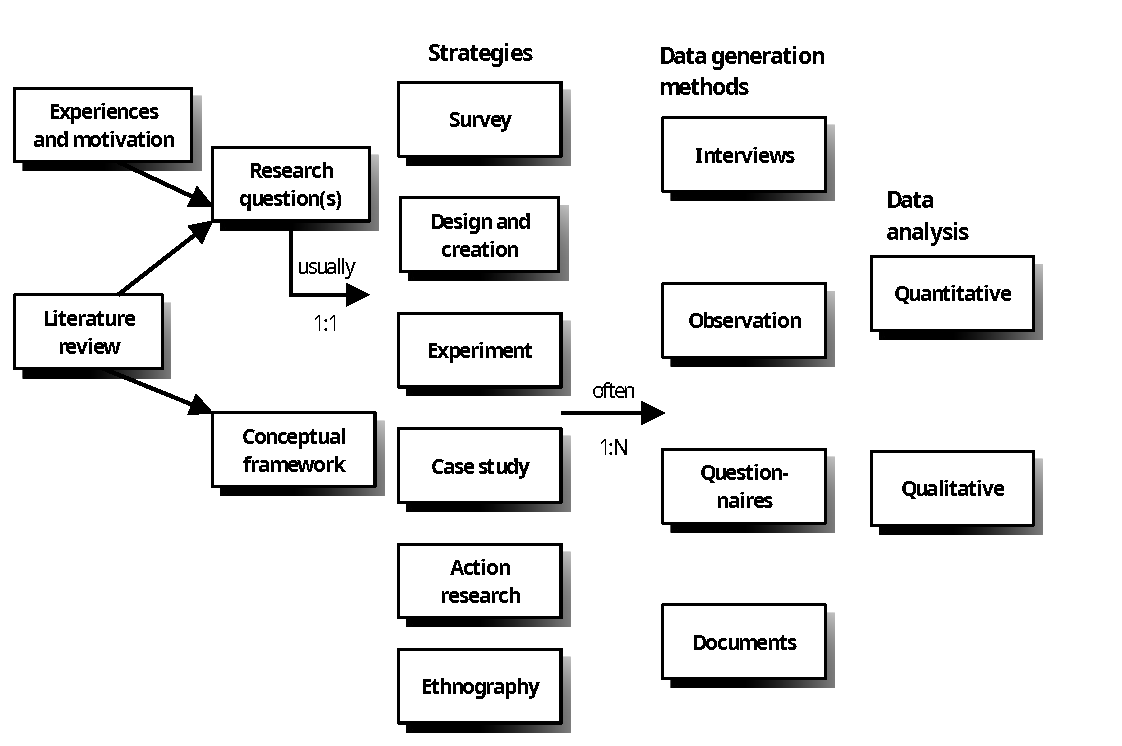
\includegraphics[width=\textwidth]{modelo_proceso.pdf}
\end{figure}
\end{frame}

\begin{frame}{Process Model}
\begin{figure}
    \centering
    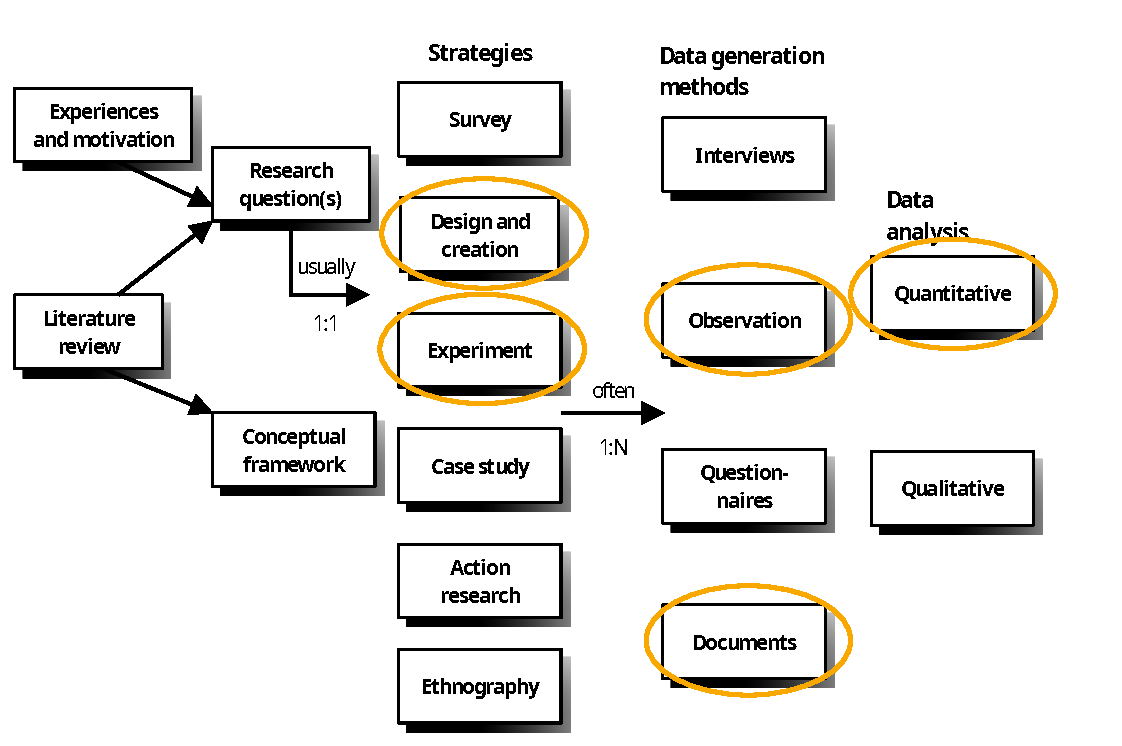
\includegraphics[width=\textwidth]{modelo_proceso_circle.pdf}
\end{figure}
\end{frame}

\begin{frame}{Process Model}

\begin{alertblock}{Literature Review}
    \smallskip
    \emph{Systematic Literature Mapping}~\cite{Petersen2007}, a process for exploring
    the situation of a wide research area with a high level of granularity.
\end{alertblock}

\begin{alertblock}{Strategy}
    \smallskip
    \emph{Engineering Design}~\cite{Dym2012}, the systematic, intelligent generation and evaluation
    of specifications for artifacts whose form and function achieve stated objectives and satisfy specified
    constraints.
\end{alertblock}

%\begin{alertblock}{Data Generation Methods}
%Observations (experiments) to evaluate preliminary products.
%\end{alertblock}

%\begin{alertblock}{Data Analysis}
%    Quantitative
%\end{alertblock}

\end{frame}

\section{State of the Art}

\begin{frame}{Systematic Literature Mapping}
\begin{figure}
    \begin{alertblock}{Questions}
        \begin{itemize}
            \item RQ1. How has the research area evolved?
            \item RQ2. What is the maturity level of the research area?
            \item RQ3. How far are we from an interactive tool that provides interactive access
                to raw data files stored in distributed storage?
        \end{itemize}
    \end{alertblock}
    \begin{block}{Search strategy}
        \begin{itemize}
            \item Set of known works from \cite{Idreos2015}
            \item Forward Snowballing
            \item Digital Libraries
            \item Two searches: 2017 and 2022
        \end{itemize}
    \end{block}
    \begin{block}{Exclusion Criteria}
        \smallskip
        Unsupported language, incomplete publication, off-topic, not primary, duplication.
    \end{block}
\end{figure}
\end{frame}

\begin{frame}{Classification}
  %\begin{columns}[t, totalwidth=1.02\textwidth]
    \metroset{block=fill}
   % \begin{column}{0.45\linewidth}
        \begin{block}{Category~\cite{Idreos2015}}
            %Three main layers:
            \begin{itemize}
                \item Database Layer
                    \begin{itemize}
                        \item Indexes, Data Storage
                    \end{itemize}
                \item Middleware
                    \begin{itemize}
                        \item Interactive Performance Optimizations
                    \end{itemize}
                \item User Interaction
                    \begin{itemize}
                        \item Data Visualization, Exploration Interfaces
                    \end{itemize}
            \end{itemize}
        \end{block}
    %\end{column}
    %\begin{column}{0.45\linewidth}
        \begin{block}{Research type~\cite{Wieringa2006}}
            \begin{itemize}
                \item Validation Research
                \item Proposal of Solution
                \item Evaluation Research
                \item Philosophical Paper
                \item Opinion Paper
            \end{itemize}
        \end{block}
    %\end{column}
    %\end{columns}
\end{frame}

\begin{frame}{}
\begin{figure}
    \centering
    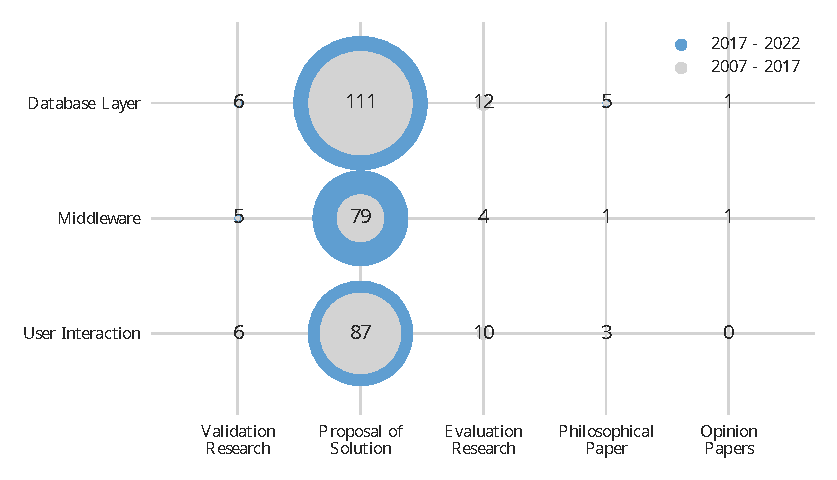
\includegraphics[width=\textwidth]{layer_vs_type.pdf}
    \caption{Layer vs. Study research type.}
\end{figure}
\end{frame}

\begin{frame}{Conclusions}
    \begin{block}{RQ1. How has the research area evolved?}
        \smallskip
        All three layers are well studied, but the middleware layer is becoming a more popular target.
    \end{block}
    \begin{block}{RQ2. What is the maturity level of the research area?}
        \smallskip
        The vast majority of studies are \emph{Proposal of Solutions}. There is very little follow-up of implementations in practice.
    \end{block}
\end{frame}

\begin{frame}{Conclusions}
    \begin{block}{RQ3. How far are we from a tool that solves our three requirements?}
        \begin{figure}
            \centering
            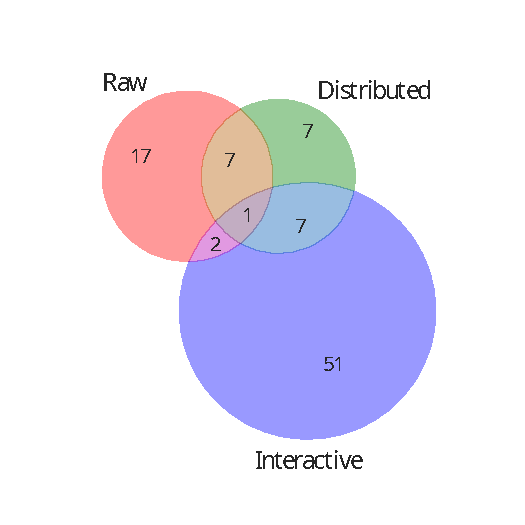
\includegraphics[width=0.6\textwidth]{venn.pdf}
        \end{figure}
    \end{block}
\end{frame}

\begin{frame}{Threats to Validity}
\begin{itemize}
    \item Lack of well-defined keywords
    \item Search bias (i.e., set of online libraries)
    \item Classification bias
\end{itemize}
\end{frame}

\begin{frame}{Insights}
    \begin{block}{}
        Most solutions treat files as separate, independent relations~\cite{Silva2016}. They offer
        little to no assistance in finding relations that \textit{overlap}: \alert{Schema Homogenization}.
    \end{block}
    \begin{block}{}
        One exception is \textsc{Kayak}~\cite{maccioni_crossing_2017}.
        \begin{itemize}
            \item Integrates \textsc{Metanome}~\cite{papenbrock2015data}.
            \item Based on \emph{Inclusion Dependencies} (IND): discrete data types.
        \end{itemize}
    \end{block}
    \begin{block}{}
        \emph{Identifying Relationships between Scientific Datasets}~\cite{alawini2016} does not
        consider multidimensional attributes
    \end{block}
    \alert{\textbf{Can we generalize IND to uncertain, multidimensional sets of attributes?}}
\end{frame}

\begin{frame}{}
\begin{figure}
    \centering
    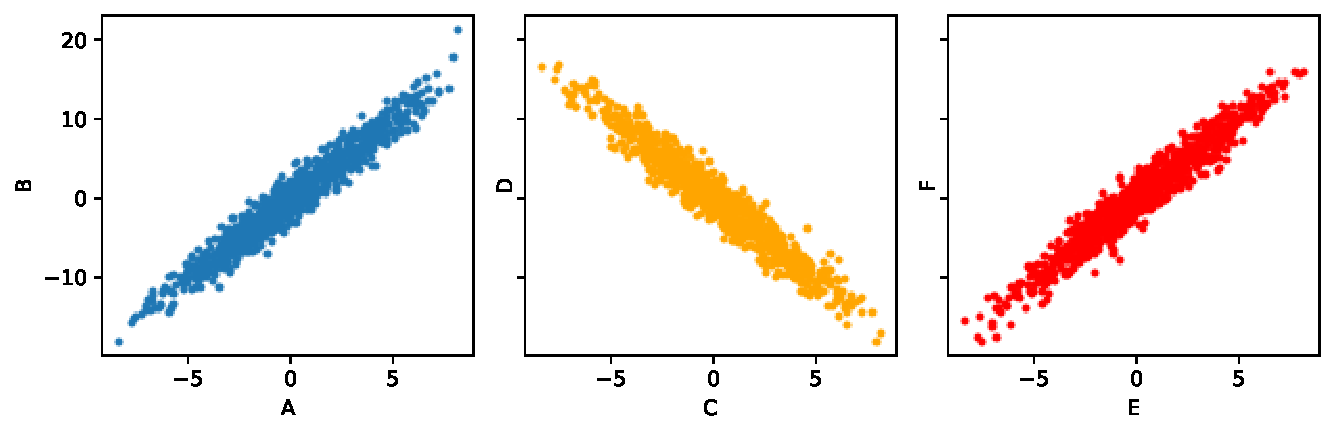
\includegraphics[width=\textwidth]{no2ind.pdf}
    \caption{Example of a 2D distribution where the pairwise matching is insufficient}
\end{figure}
\end{frame}

\section{\PresQ}

\subsection{Background}

\begin{frame}{IND vs EDD}
    \begin{block}{Inclusion Dependency (IND)}
        \smallskip
        An inclusion dependency between column A of relation
        R and column B of relation S, written $R.A \subseteq S.B$, asserts that each
        value of A appears in B. Similarly, for two sets of columns X
        and Y , we write $R.X \subseteq S.Y$ , or $X \subseteq Y$ , when each distinct
        combination of values in X appears in Y~\cite{abedjan2015}
    \end{block}
    \begin{block}{\alert{Equally-Distributed Dependency (EDD)}}
        \smallskip
        An equally-distributed dependency between a set of columns X
        of relation R and a set of columns Y of relation S, written $R.X \eqdist S.Y$ or
        $X \eqdist Y$, asserts that the values of X and Y follow the same probability distribution.
    \end{block}
\end{frame}

\begin{frame}{Inference Rules}
    \metroset{block=fill}
    \begin{block}{Reflexivity}
        $R[X] \eqdist R[X]$
    \end{block}
    \begin{block}{Permutation and projection}
        If $R[A_1,\dots,A_n] \eqdist S[B_1,\dots,B_n]$ then
        $R[A_{i_1},\dots,A_{i_m}] \eqdist S[B_{i_1},\dots,B_{i_m}]$ for each sequence
        $i_1,\dots,i_m$ of distinct integers from $\{1,\dots,n\}$
    \end{block}
    \begin{block}{Transitivity}
        $ R[X] \eqdist S[Y] \land S[Y] \eqdist T[Z] \implies R[X] \eqdist T[Z]$
    \end{block}
    
    \metroset{block=transparent}
    \begin{block}{}
    The reflexivity, permutation, and transitivity rules are well-known to hold
    for $\eqdist$ \cite{randles1979introduction}.

    For the projection, see \alert{Section 5.1, Proof 1} (page 53).
    \end{block}
\end{frame}

\begin{frame}{Search Space}
    \metroset{block=fill}
    \begin{block}{Partial Order}
        Let $I_1 = R[X] \eqdist S[Y]$ and $I_2 = R'[X'] \eqdist S'[Y']$.
        
        $I_1$ \textbf{specializes} $I_2$ (denoted $I_1 \prec I_2)$ iff
        \begin{enumerate}
            \item $R = R'$ and $S = S'$.
            \item $X$ and $Y$ are sub-sequences of $X'$ and $Y'$, respectively.
        \end{enumerate}
    \end{block}

    \begin{block}{Satisfiability}
    Let $I = R[X] \eqdist S[Y]$.
    A dataset $d$ \emph{satisfies} $I$ iff  a statistical test fails to reject $H_0: P(R[X]) = P(S[Y])$
    given a significance level $\alpha$.
    This is denoted as $d \models I$.
    \end{block}
\end{frame}

\begin{frame}{Search Space}
\begin{figure}
    \centering
    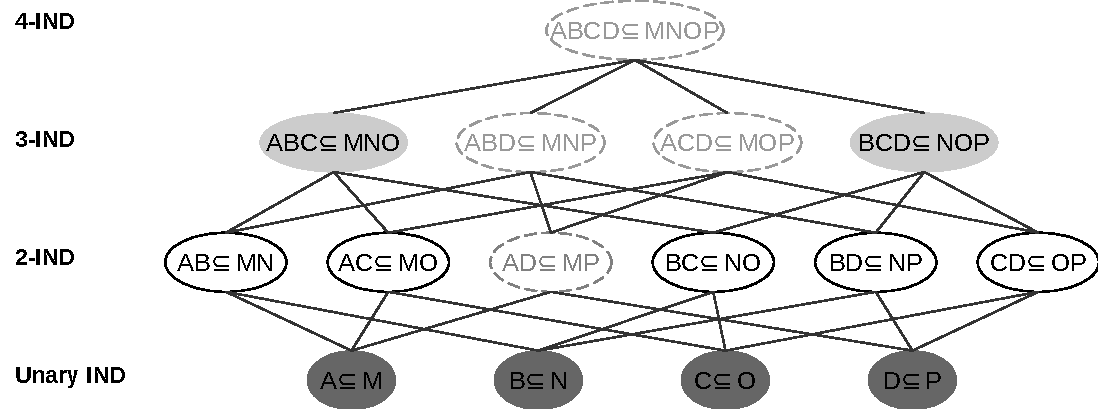
\includegraphics[width=\textwidth]{lattice.pdf}
    \caption{Search space for INDs}
\end{figure}
\end{frame}

\begin{frame}{Traversal}
    Given $I_1 \prec I_2$:
    
    \begin{enumerate}
        \item If $d \models I_2$, then $d \models I_1$ (If we can not reject $H_{0_2}$, we can not reject $H_{0_1}$.)
        \item $d \not\models I_1$ with a probability $\alpha$ when $d \models I_2$
            (Rejecting $H_{0_1}$ \emph{does not} imply the rejection of $H_{0_2}$)
    \end{enumerate}
\end{frame}

\begin{frame}{Traversal}
    \begin{exampleblock}{Example}
    \smallskip
    If we have two sets of $10$ attributes that are equally distributed, the number of
    3-dimensional projections (specializations) that must be equally distributed will be $\binom{10}{3} = 120$.
    If we have a significance level of $\alpha = 0.1$, the expected number of
    falsely rejected 3-dimensional equalities is then $12$.
    \end{exampleblock}
\end{frame}


\begin{frame}{Bottom-Up Search}
    \begin{block}{Naive Traversal of the Search Space}
        \smallskip
        We can validate pairwise EDDs. Then, we build possible three-wise EDD and validate them.
        Then, we build possible four-wise EDD...
    \end{block}
        
    \begin{alertblock}{Complexity}
    \smallskip
    Generally, if we have an n-EDD between two datasets, and traverse the lattice bottom-up, we need
    to test...
    
    \begin{equation*}
        \sum_{k=1}^{n}{\binom{n}{k}} = \sum_{k=1}^{n} \frac{n!}{n!(n - k)!}
    \end{equation*}
    
    possible combinations of attributes.
    \end{alertblock}
\end{frame}

\begin{frame}{Complexity}

    It turns out that finding INDs/EDDs is one of the hardest computer science
    problems~\cite{Blsius2017}.
    
    \begin{itemize}
        \item It is \textbf{NP-hard}.
        \item The \textbf{number of solutions} can be \textbf{exponential} in the input size.
        \item It is \textbf{non-approximable} (NP-hard even if we accept an error margin).
    \end{itemize}
    
    \bigskip
    
    However, the run-time can be reasonable if we are optimistic: i.e. if we assume
    $n$ 1-EDDs are derived from a single $n$-EDD, we only need one test: Top-down traversal.
    
    \bigskip
    
    But we risk being too optimistic and needing to traverse the full search space from top to bottom.
\end{frame}

\subsection{Clique Finding}
\begin{frame}{Clique Finding}
    The problem can be mapped to finding cliques on hypergraphs: \textsc{Find2}~\cite{koeller2003discovery}:
    
    \begin{enumerate}
        \item Pairwise matches (1EDD) are mapped to \textbf{nodes}.
        \item $k$-combinations of 1EDD are mapped to \textbf{$k$-edges}.
        \item Cliques of size $n$ \emph{may} correspond to $n$-EDD.
        \item If they do not, we \emph{break} these cliques into a set of $k+1$ edges and
            validate them.
    \end{enumerate}

    The search space is traversed alternating between bottom-up \emph{and} top-down.
\end{frame}

\begin{frame}{Clique Finding}
    \begin{exampleblock}{Example}
        \begin{columns}
        \begin{column}{.7\textwidth}
        \begin{enumerate}
            \item $A \eqdist M, B \eqdist N, C \eqdist O, D \eqdist P$
            \item All 6 possible 2-EDD are true
            \item Clique with 4 nodes $ABCD \eqdist MNOP$
            \item If false, we break it into
                \begin{enumerate}
                    \item $ABC \eqdist MNO$
                    \item $BCD \eqdist NOP$
                    \item $ACD \eqdist MOP$
                    \item \ldots
                \end{enumerate}
        \end{enumerate}
        \end{column}
        \begin{column}{.3\textwidth}
            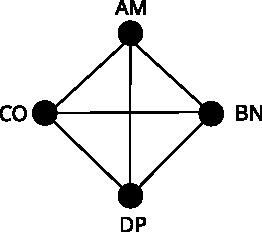
\includegraphics[width=\linewidth]{4clique}
        \end{column}
        \end{columns}
    \end{exampleblock}
    
    \pause
    
    \begin{alertblock}{}
    But we are using statistical tests.
    
    \begin{itemize}
        \item We may falsely refuse an EDD (type I error)
        \item Or falsely accept it (type II error).
    \end{itemize}
    \end{alertblock}
\end{frame}


\subsection{Quasi-Clique Finding}
\begin{frame}{Quasi-Clique Finding}
    \metroset{block=fill}
    \begin{alertblock}{Definition}
    Given a k-uniform hypergraph $(V,E)$, and two parameters $\lambda, \gamma \in [0,1]$,
    the sub-graph $H'=(V',E')$ induced by a subset $V' \subseteq V$ is a
    $(\lambda-\gamma)$ quasi-clique iff:
    
    \begin{equation}
        |E'| \ge \gamma \cdot \binom{|V'|}{k}
        \label{eq:edge_hyperclique}
    \end{equation}
    
    \begin{equation}
        \forall v \in V': deg_{V'}(v) \ge \lambda \cdot \binom{|V'| - 1}{k - 1}
        \label{eq:deg_hyperclique}
    \end{equation}

    Where $deg_{V'}(v)$ represents the degree of $v$, and $E'$ is a subset of $E$ such that
    $\forall e \in E' : e \subseteq V'$
    \end{alertblock}
    
    We can approximate $\gamma \approx 1 - \alpha$. How do we bound $\lambda$?
\end{frame}

\begin{frame}{Quasi-Clique Finding}
    \begin{block}{}
    There is no reason to think that any particular subset of the edges
    has a higher probability of having missing members. If a given node has an
    unexpectedly low degree, it is most likely connected by spurious edges.
    \end{block}
    \metroset{block=fill}
    \begin{block}{The degree should follow a hypergeometric distribution}
    \begin{equation}
        \forall v \in V': \operatorname{CDF}(\operatorname{Degree}(v)) \ge \Lambda
    \end{equation}
    \end{block}
    \centering
    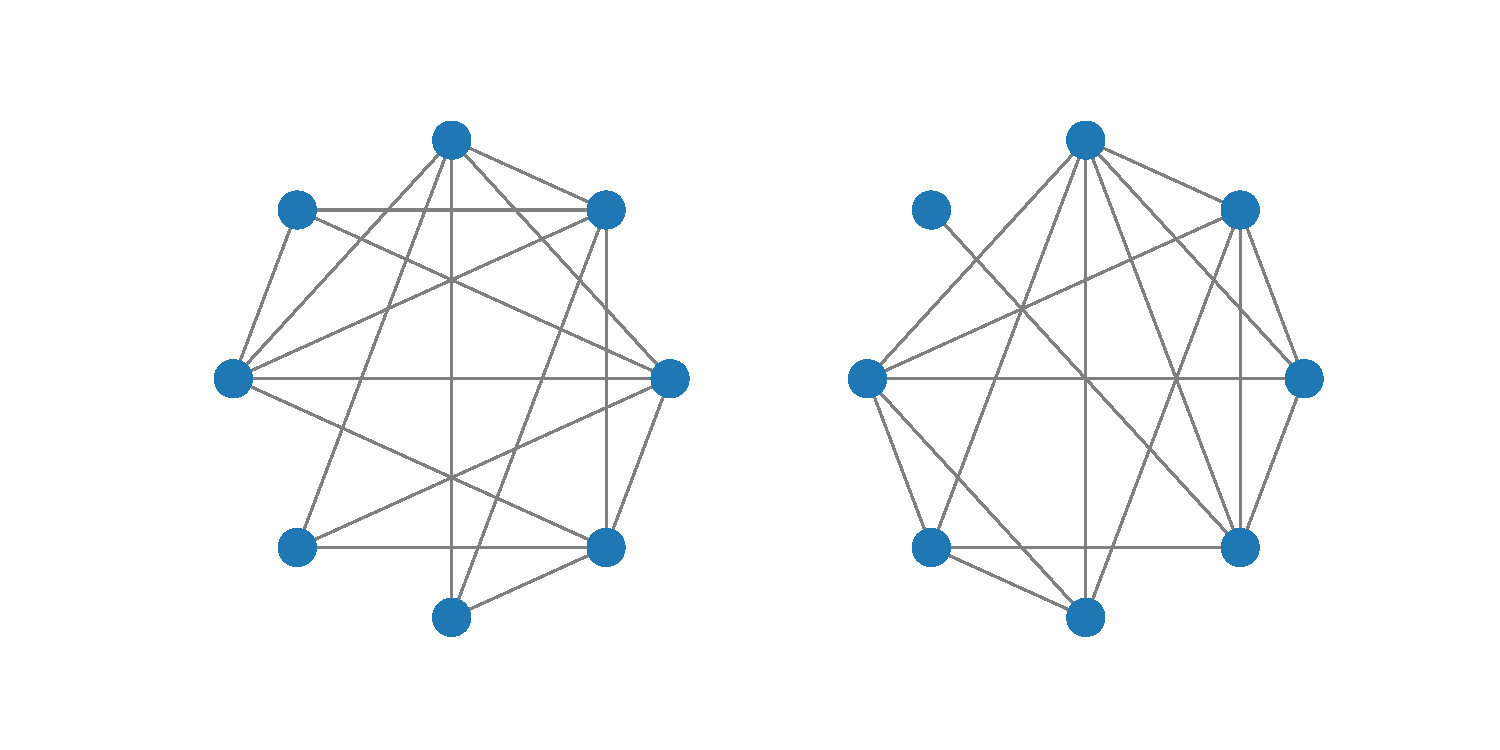
\includegraphics[width=0.6\linewidth]{quasicliques}
\end{frame}

\begin{frame}{\PresQ}

    \begin{block}{}
    \PresQ~\cite{AlvarezAyllonPresQ2022} is an algorithm for finding quasi-cliques on uniform
    $k$-hypergraphs.
    
    \begin{enumerate}
        \item Finds ``seeds'' using a modified version of \textsc{Hyperclique}~\cite{koeller2003discovery}.
        \item Grows the ``seeds'' following a tree-shaped, depth-first
        traversal~\cite{uno_efficient_2010}.
    \end{enumerate}
    \end{block}
    
    \begin{alertblock}{Complexity}
        \smallskip
        The number of maximal cliques is bound in general by $\Omega(a^{|V|/b})$,
        where $a, b$ are two constants that depend on the rank of the hypergraph~\cite{Tomescu1981}.
        
        The worst-case is always going to be exponential.
    \end{alertblock}
\end{frame}

\subsection{Algorithm}

\begin{frame}{}
    \begin{columns}
    \begin{column}{0.5\linewidth}
        \renewcommand{\theenumi}{\alph{enumi}}
        \begin{enumerate}
            \item Generate candidate 1EDD.
            \item If $\eqdist$ can not be rejected, map to nodes.
            \item Test all pairwise combinations (2EDD).
            \item If $\eqdist$ can not be rejected, map to edges on a $k$-hypergraph.
            \item Search for quasi-cliques\label{step:search_quasi}.
            \item Validate quasi-cliques.
            \item Rejected quasi-cliques are used to generate a $k+1$-hypergraph.
            \item Go-to \ref{step:search_quasi}.
        \end{enumerate}
    \end{column}
    \begin{column}{.5\linewidth}
        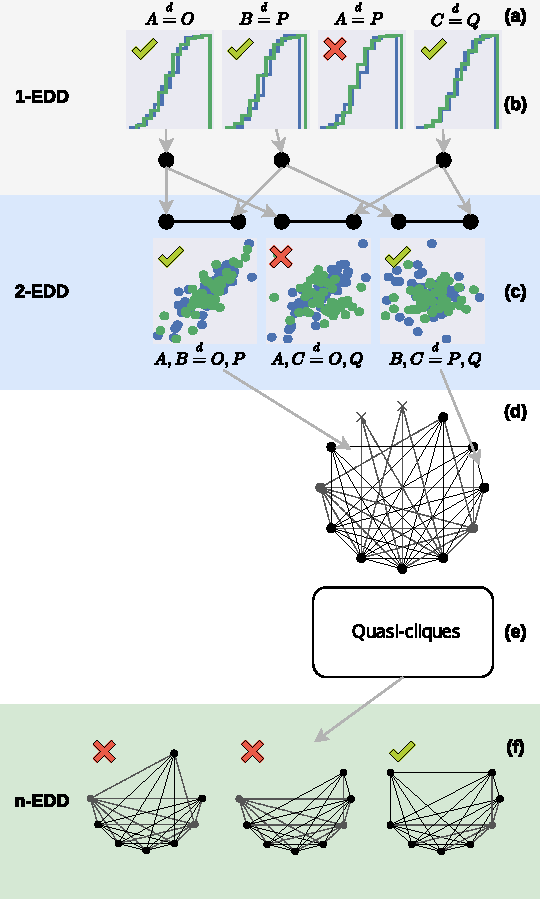
\includegraphics[width=0.9\linewidth]{pipeline}
    \end{column}
    \end{columns}
\end{frame}

\section{\PresQ Experiments}

\begin{frame}{Clique Recovery: Missing Edges}
    \begin{figure}
        \centering
        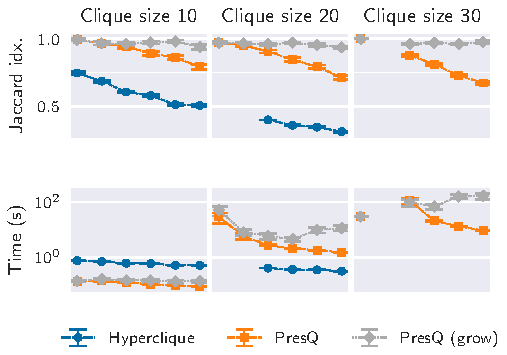
\includegraphics{3hyper_alpha}
        \caption{Robustness wrt. missing edges (3-hypergraph)}
    \end{figure}
\end{frame}

\begin{frame}{Clique Recovery: Spurious Edges}
    \begin{figure}
        \centering
        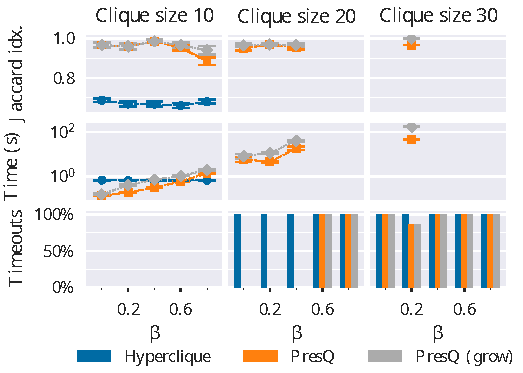
\includegraphics{3hyper_beta}
        \caption{Robustness wrt. spurious edges (3-hypergraph)}
    \end{figure}
\end{frame}

\begin{frame}{Clique Recovery: Correlated Missing / Spurious}
\begin{figure}
    \centering
    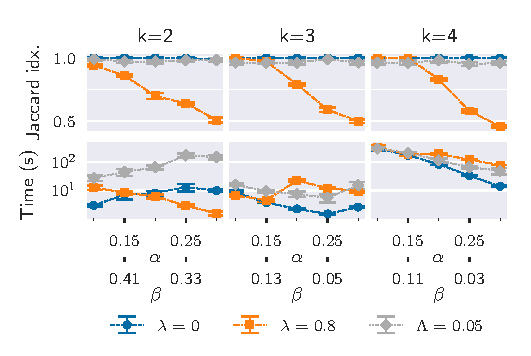
\includegraphics{quasi_corr_20}
    \caption{
    Recovery ratio and run-times for cliques of size 20 on uniform $(2,3,4)$-hypergraphs.
    }
\end{figure}
\end{frame}

\begin{frame}{EDD Finding}
\begin{figure}
    \centering
    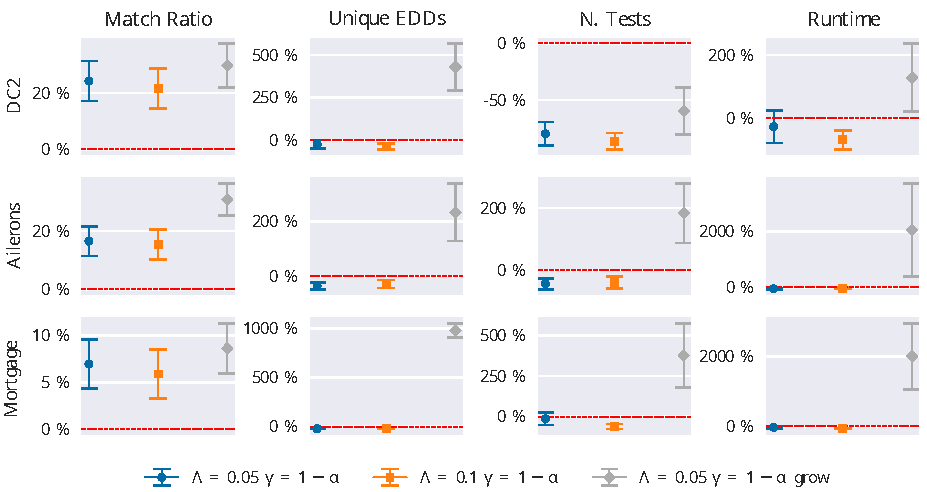
\includegraphics[width=\textwidth]{all}
    \caption{$95\%$ confidence intervals for the percent difference
    between \textsc{Find} and \PresQ.}
\end{figure}
\end{frame}

\begin{frame}{Insights Only From the Data}
\begin{figure}
    \centering
    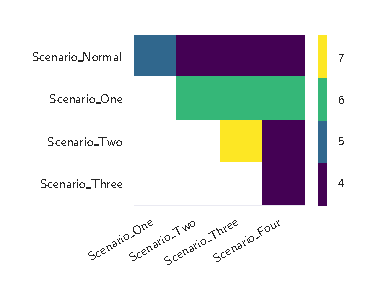
\includegraphics{afds}
    \caption{
        Pairwise max arity found on the \emph{Aircraft Fuel Distribution System} dataset for each pair of scenarios.
        Without even knowing the structure or content of the files, we can see that
        scenarios two and three are the most similar, which we can confirm in the
        original paper~\cite{Gheraibia2019}.
    }
\end{figure}
\end{frame}

\section{Two-Sample Test Based on Self-Organizing Maps}

\subsection{Background}

\begin{frame}{Classifier 2-Sample Tests}
    \begin{block}{}
        A binary classifier can be seen as a two-sample test.
        If a classifier has a better-than-chance performance (50\%), the two classes do not originate from the same
        population~\cite{friedman2004multivariate}.
        \smallskip
        Given two samples $P$ and $Q$:
        \begin{enumerate}
            \item Label samples originating from $P$ with $1$, and those originating from $Q$ with $-1$.
            \item Pool both samples into a single set $U$
        \end{enumerate}
    \end{block}
\end{frame}

\begin{frame}{Classifier 2-Sample Tests}
    \metroset{block=fill}
    \begin{block}{Approach 1~\cite{friedman2004multivariate}}
        A classifier is trained on $U$ to predict the label. The classifier score function $F(u)$ is used
        to reduce the n-dimensional statistical test to a 1-dimensional statistical test.
    \end{block}
    \begin{block}{Approach 2~\cite{lopez2016revisiting}}
        $U$ is split into training and test sets. The accuracy of the classifier on the test set is the test statistic.
    \end{block}
\end{frame}

\begin{frame}{Self-Organizing Maps}
    An \emph{unsupervised} machine-learning algorithm that learns
    a projection from a high-dimension input space into a low-dimension output space.

    \smallskip
    
    The output space is modeled as a grid of \emph{neurons} that \emph{responds} to a set of
    values from the input space~\cite{kohonen1982self}.

    \smallskip
    
    \alert{The output model preserves the topology of the input space}: any continuous changes
    in the input data cause a continuous change on the neural map~\cite{Villmann1999}.
    
    \metroset{block=fill}
    \begin{alertblock}{Insight}
        \smallskip
        If two samples are equally distributed on the input space, they must be equally distributed on the output space.
    \end{alertblock}    
\end{frame}

\subsection{Algorithm}

\begin{frame}{SOM 2-Sample Test}
    \begin{block}{Algorithm}
        \begin{enumerate}
        \item Train a SOM $M$ of size $(w, h)$ over $U = X \cup Z$.
        \item Project $X$ and $Z$ separately over the SOM  $M$.
        \item For each neuron $n_i$, count how many points from $X$ ($R_i)$ and how many from $Z$ ($S_i)$ are mapped to it.
        \item Perform a $\chi^2$ two-sample test.
        \end{enumerate}

        Under the null hypothesis, the test statistic follows a $\chi^2$ distribution with $k - c$ degrees of freedom,
        \begin{itemize}
            \item $k$ is the number of cells (neurons) where ${R_i + S_i > 0}$
            \item $c = 1$ if the sample sizes are equal, or $c = 0$ otherwise~\cite{press1993numerical}.
        \end{itemize}        
    \end{block}
\end{frame}

\begin{frame}{Advantages}
    \begin{itemize}
        \item After the test, we have a trained model that can be used for
            
            \begin{itemize}
                \item Visualization
                \item Clustering~\cite{ultsch2005esom}
            \end{itemize}

        \item The full dataset is used.
        \item It works with unbalanced sample sizes from $X$ and $Z$.
        \item It can be generalized to non-vectorial data~\cite{kohonen1982self}.
    \end{itemize}
\end{frame}

\subsection{Experiments}

\begin{frame}{Experiment: Multidimensional Normal Distribution}
    \begin{block}{Evaluated Alternatives}
        \smallskip
        \begin{itemize}
            \item Nearest neighbor type coincidences~\cite{Henze1988, Schilling1986b}.
            \item Classifier two-sample tests~\cite{lopez2016revisiting}.
        \end{itemize}
    \end{block}
    \begin{block}{``Fair'' Distributions}
        \smallskip
        \cite{ramdas2015decreasing} argue that a ``fair'' evaluation of the
        statistical power as the dimensionality increases must keep the
        amount of information fixed.
    \end{block}
\end{frame}

\begin{frame}{}
\begin{figure}
    \centering
    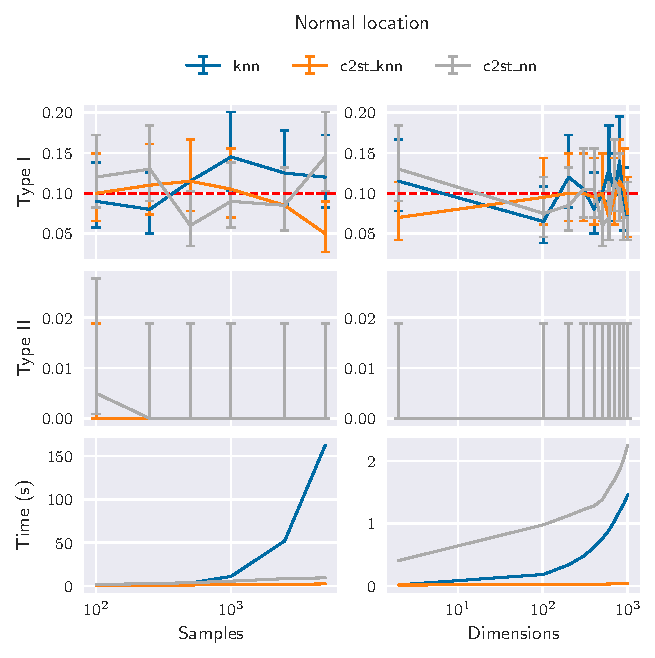
\includegraphics[height=\textheight]{normal_location}
\end{figure}
\end{frame}

\begin{frame}{}
\begin{figure}
    \centering
    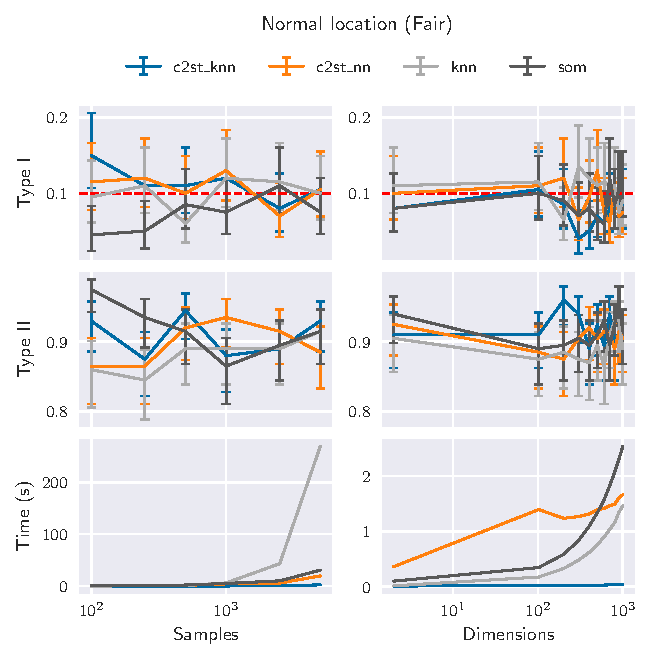
\includegraphics[height=\textheight]{normal_location_fair}
\end{figure}
\end{frame}

\begin{frame}{Experiment: Eye Movement Dataset}
    \begin{block}{Dataset}
        \smallskip
        11 subjects were shown a question and a list of ten 
        sentences: one correct answer (C), four relevant for the question (R), and five irrelevant (I).
        
        Their eye movement was measured for each answer and summarized into 22 features~\cite{salojarvi2005inferring}.
    \end{block}
    \begin{block}{Evaluated Alternatives}
        \smallskip
        \begin{itemize}
            \item Nearest neighbor type coincidences~\cite{Henze1988, Schilling1986b}.
            \item Classifier two-sample tests~\cite{lopez2016revisiting}.
            \item Kernel-Based methods MMD-B~\cite{zaremba2013b} and Song's~\cite{song2021fast}.
        \end{itemize}
    \end{block}
\end{frame}

\begin{frame}{}
\begin{table}[htbp]
    \centering
    \begin{tabular}{c r r r r r r}
        \hline
        \multicolumn{7}{c}{\thead{I vs. C}} \\
        \hline
        \thead{m = n} & \thead{Song} & \thead{MMD-B} & \thead{KNN} & \thead{C2ST-KNN} & \thead{C2ST-NN} & \thead{SOM} \\
        \hline
        100 & 0.826 & 0.374 & \textbf{0.973} & 0.164 & 0.079 & 0.042 \\
        200 & 0.998 & 0.850 & \textbf{1.000} & 0.565 & 0.349 & 0.947 \\
        300 & \textbf{1.000} & 0.985 & \textbf{1.000} & 0.863 & 0.644 & \textbf{1.000} \\
        400 & \textbf{1.000} & \textbf{1.000} & \textbf{1.000} & 0.968 & 0.882 & \textbf{1.000} \\
        \\
        \hline
        \multicolumn{7}{c}{\thead{R vs. C}} \\
        \hline
        \thead{m = n} & \thead{Song} & \thead{MMD-B} & \thead{KNN} & \thead{C2ST-KNN} & \thead{C2ST-NN} & \thead{SOM} \\
        \hline
        100 & 0.670 & 0.236 & \textbf{0.845} & 0.062 & 0.023 & 0.007 \\
        200 & 0.969 & 0.685 & \textbf{0.996} & 0.298 & 0.139 & 0.672 \\
        300 & 0.999 & 0.941 & \textbf{1.000} & 0.558 & 0.314 & 0.987 \\
        400 & \textbf{1.000} & 0.988 & \textbf{1.000} & 0.811 & 0.560 & \textbf{1.000} \\
    \end{tabular}
    \caption{Empirical statistical power for the eye movement datasets.}
    \label{tab:eye}
\end{table}
\end{frame}

\begin{frame}{Interpretability}
    \begin{figure}
        \centering
        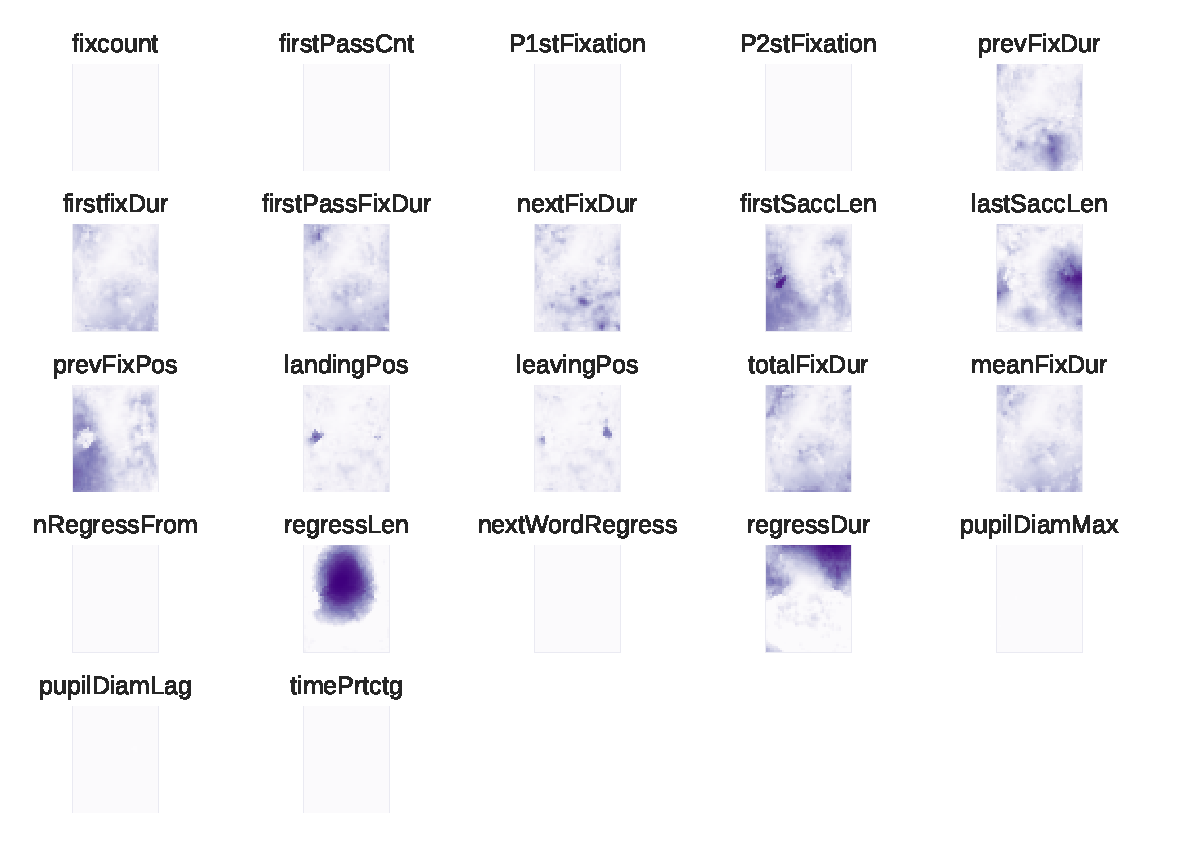
\includegraphics[trim=5pt 75pt 5pt 5pt,clip,width=0.9\textwidth]{eye_features.eps}
        \caption{
            The features ``Regression length'' and ``regression duration'' stand out.
            They are related to re-reading a word, which is expected to happen when reading a correct answer~\cite{salojarvi2005inferring}.
        }
    \end{figure}
\end{frame}


\begin{frame}{Caveat}
    Rosenblatt~\cite{rosenblatt2019better} argue that provable test statistics
    should be preferred over heuristic alternatives.
    \smallskip
    Our proposal is oriented toward \alert{exploring} abundant structured data.
    Developing a tailored statistic for all possible combinations is not viable,
    and a pragmatic approach is more suitable~\cite{kim2021classification}.
\end{frame}

\section{Threats to Validity}

\begin{frame}{Internal Validity}
    \begin{alertblock}{Significance of the Results}
        \smallskip
        The presented results could be a statistical fluctuation. To reduce the risk:
        
        \begin{itemize}
            \item We have taken multiple measures with randomized initial conditions.
            \item We have reported either 95\% confidence intervals or quartiles to make the measure errors explicit.
        \end{itemize}
    \end{alertblock}
\end{frame}

\begin{frame}{Internal Validity}
    \begin{alertblock}{Implementation Bias}
        \smallskip
        The evaluated \PresQ and \textsc{Find} implementations share most parts of the code. The differences can only originate
        from the algorithms and not the implementations.
        
        \smallskip
        
        For the statistical tests, SOM, $k$NN, C2ST-NN and C2ST-kNN have all been implemented using well known
        Python libraries (\textsc{somoclu}, \textsc{numpy}, \textsc{scikit-learn}).
    \end{alertblock}
\end{frame}

\begin{frame}{External Validity}
    \begin{alertblock}{Generalization of the results}
        \smallskip
        We have performed tests with a multitude of datasets from different domains.
        
        \smallskip

        For the SOM statistical test, in the interests of transparency, we have incorporated a set
        of ``fair'' tests explicitly designed to show the shortcomings of multidimensional statistical tests~\cite{ramdas2015decreasing}.
        
    \end{alertblock}
\end{frame}

\section{Conclusions}

%\begin{frame}{Contributions}
%    \begin{alertblock}{Survey of the State of the Art}
%        \smallskip
%        Contribute to the first sub-objective: finding existing techniques that help users to explore the data \emph{in-situ}.
%    \end{alertblock}

%    \begin{block}{New category for IDE: \alert{Schema Homogenization}}
%        \smallskip
%        Contributes to the first and second sub-objectives: identify gaps in the coverage.
%    \end{block}

%    \begin{alertblock}{Equally-Distributed Dependency}
%        \smallskip
%        Contributes to the second sub-objective: identify gaps in the coverage.
%    \end{alertblock}
%\end{frame}

%\begin{frame}{Contributions: Algorithms}
%    \begin{alertblock}{\PresQ}
%        \smallskip
%        It can be used to find sets of Equally-Distributed attributes between datasets.
%        The Quasi-clique component can potentially be of use to other areas such as
%        chemistry or biology~\cite{Bretto2013}.
%    \end{alertblock}

%    \begin{alertblock}{Two-Sample Test Based on SOM}
%        \smallskip
%        A statistical test with a performance comparable to other tests based on machine learning models,
%        with an interpretable output.
%    \end{alertblock}

%    \begin{block}{}
%    These two algorithms contribute to the third sub-objective: design new algorithms tailored to numerical and
%    uncertain data.
%    \end{block}
%\end{frame}

\begin{frame}{Contributions}

\begin{alertblock}{\emoji{check-mark} Find existing techniques that help users to explore the data in situ}
    \begin{itemize}
        \item Survey of the State of the Art
    \end{itemize}
\end{alertblock}

\begin{alertblock}{\emoji{check-mark} Identify gaps in the coverage of the existing techniques}
    \begin{itemize}
        \item New category for IDE: \alert{Schema Homogenization}
        \item Equally-Distributed Dependency
    \end{itemize}
\end{alertblock}

\begin{alertblock}{\emoji{check-mark} Design new algorithms tailored to numerical and uncertain data}
    \begin{itemize}
        \item \PresQ
        \item Two-Sample Test Based on SOM
    \end{itemize}
\end{alertblock}

\end{frame}

\begin{frame}{Contributions}

\metroset{block=fill}
\begin{block}{\emoji{white-check-mark} Main Objective}
    The proposed algorithms can assist data scientists in identifying relationships
    between numerical, raw datasets distributed across multiple files
    based solely on their intrinsic distribution.
\end{block}

\end{frame}


\begin{frame}{Future Work}
    \begin{itemize}
        \item Improve the quasi-clique finding algorithm.
                
        \item Data-aware quasi-clique finding algorithms.
        
        \item \alert{Partial equality-of-distribution}
                
        \item A Bayesian EDD finding algorithm (i.e., prior support, partial EDD~\cite{soriano2015bayesian}).
        
        \item Dimensionality reduction before EDD finding.
            
        \item \alert{Multidimensional \emph{complementarity}} (i.e., a dataset may be split 
        based on the values from a given set of attributes).

        \item Applications on privacy-preserving data mining.
    \end{itemize}
\end{frame}

\definecolor{myblue}{RGB}{35,55,59}
{\setbeamercolor{palette primary}{fg=white, bg=myblue}
\begin{frame}[standout]
  \huge Questions?
\end{frame}
}


\begin{frame}[allowframebreaks]{Bibliography}
\printbibliography[]
\end{frame}

\appendix

{\setbeamercolor{palette primary}{fg=white, bg=black}
\begin{frame}[standout]
  Backup slides
\end{frame}
}


\begin{frame}{}
\begin{figure}
    \centering
    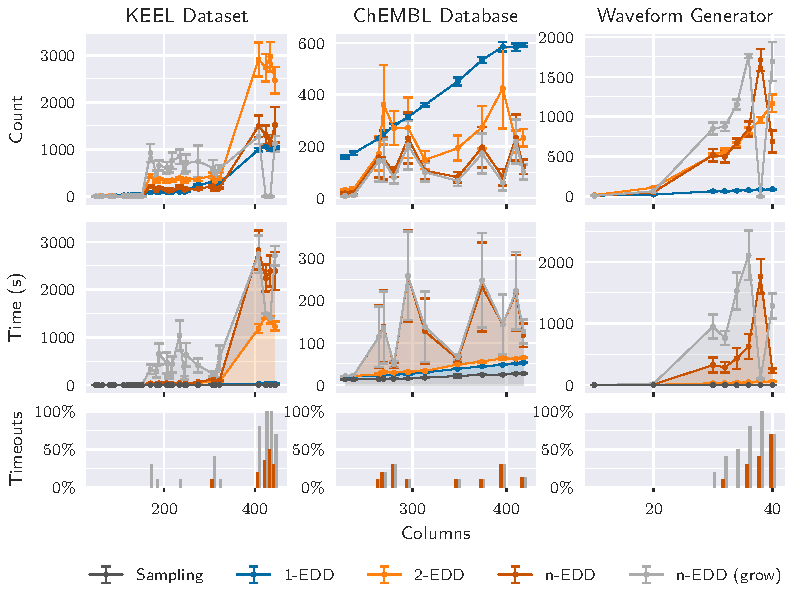
\includegraphics[width=\textwidth]{scalability.pdf}
\end{figure}
\end{frame}

\begin{frame}{}
\begin{figure}
    \centering
    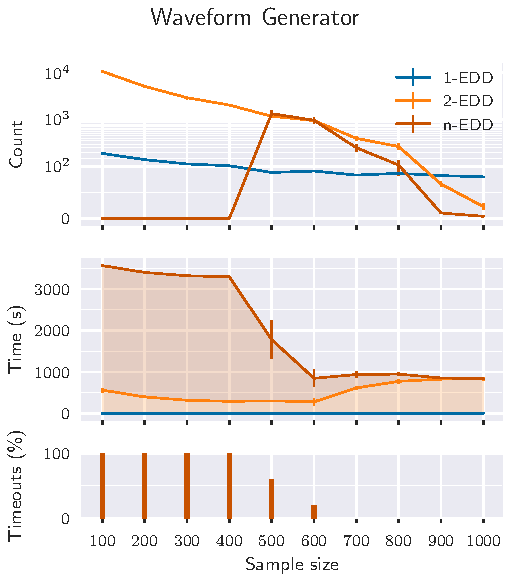
\includegraphics[height=\textheight]{scalability_sample_wave.pdf}
\end{figure}
\end{frame}

\begin{frame}{}
\begin{figure}
    \centering
    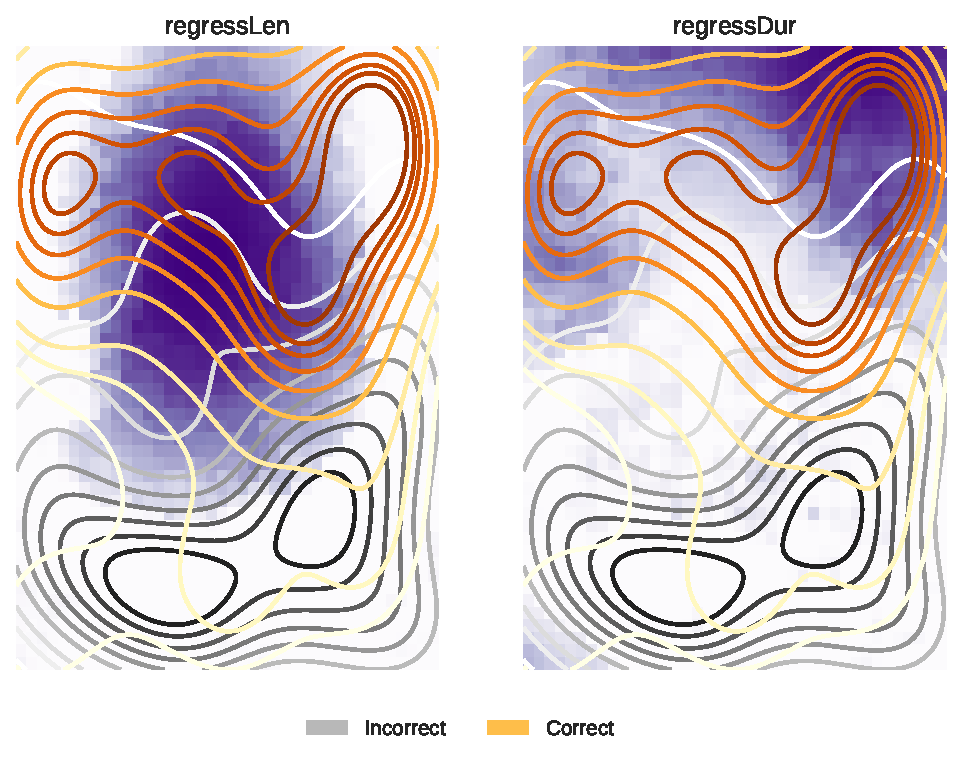
\includegraphics[height=\textheight]{eye_regress-eps-converted-to.pdf}
\end{figure}
\end{frame}

\end{document}
